\documentclass[a4paper, titlepage]{jsarticle}

\usepackage[dvipdfmx]{graphicx}
\usepackage[dvipdfmx]{hyperref}
\usepackage{pxjahyper}
\usepackage{amsmath}
\usepackage{mathtools}
\usepackage{listings}

\lstset{
  basicstyle={\ttfamily},
  identifierstyle={\small},
  commentstyle={\smallitshape},
  keywordstyle={\small\bfseries},
  ndkeywordstyle={\small},
  stringstyle={\small\ttfamily},
  frame={tb},
  breaklines=true,
  columns=[l]{fullflexible},
  numbers=left,
  xrightmargin=0zw,
  xleftmargin=3zw,
  numberstyle={\scriptsize},
  stepnumber=1,
  numbersep=1zw,
  lineskip=-0.5ex
}

\title{シミュレーション工学Ⅱ ラグランジュ補間}
\author{三浦夢生}
\date{2020年12月15日}

\begin{document}
	\maketitle

	\section{目的}
	連立方程式の解を関数補間によって求める方法について学び,理解を深める.

	ラグランジュ補間を実装する.
	
	\section{用語}
	今回用いた手法などについて簡単に説明を行う.

	\subsection{関数補間}
	ある離散的なデータが与えられているときに,そのデータ点を通る多項式を求めることでその間に存在するであろうデータを予測し,近似することを関数補間という.いくつかの方法があるうち,今回はラグランジュ補間についてまとめる.

	\subsection{ラグランジュ補間}
	2点のデータ点が与えられると一次式が定まる.同様に3点が与えられると二次式が定まる.一般に,x座標がそれぞれ異なるn個のデータ点が与えられた時n-1次式が定まる.

	この考えのもと,以下の式を用いて多項式補間をする方法を,ラグランジュ補間という.

	\begin{align}
		L(x)={\sum_{i=0}^{n}}f(x_i)l_i(x) \\
		l_i(x)={\prod_{j{\neq}i}^{n}}{\frac{x-{x_j}}{{x_i}-{x_j}}}
	\end{align}

	一次式$y={a_1}x+{a_0}$に対して$(x_0, y_0),(x_1, y_1)$を代入し,それぞれの係数について解くと
	\begin{equation}
		y={\frac{x-{x_1}}{{x_0}-{x_1}}}y_0+{\frac{x-{x_0}}{{x_1}-{x_0}}}y_1
	\end{equation}
	となる.同様に二次,三次と拡張し,係数部と全体の式を総和及び総乗の記号を用いることで上記の一般式が導出できる.

	\section{課題}
	\subsection{課題1}
	$(x,y)=(1,1),(3,2),(4,5)$を通る曲線をラグランジュ補間によって求め,区間$[-1,5]$のグラフを示す.

	\begin{figure}[ht]
		\centering
		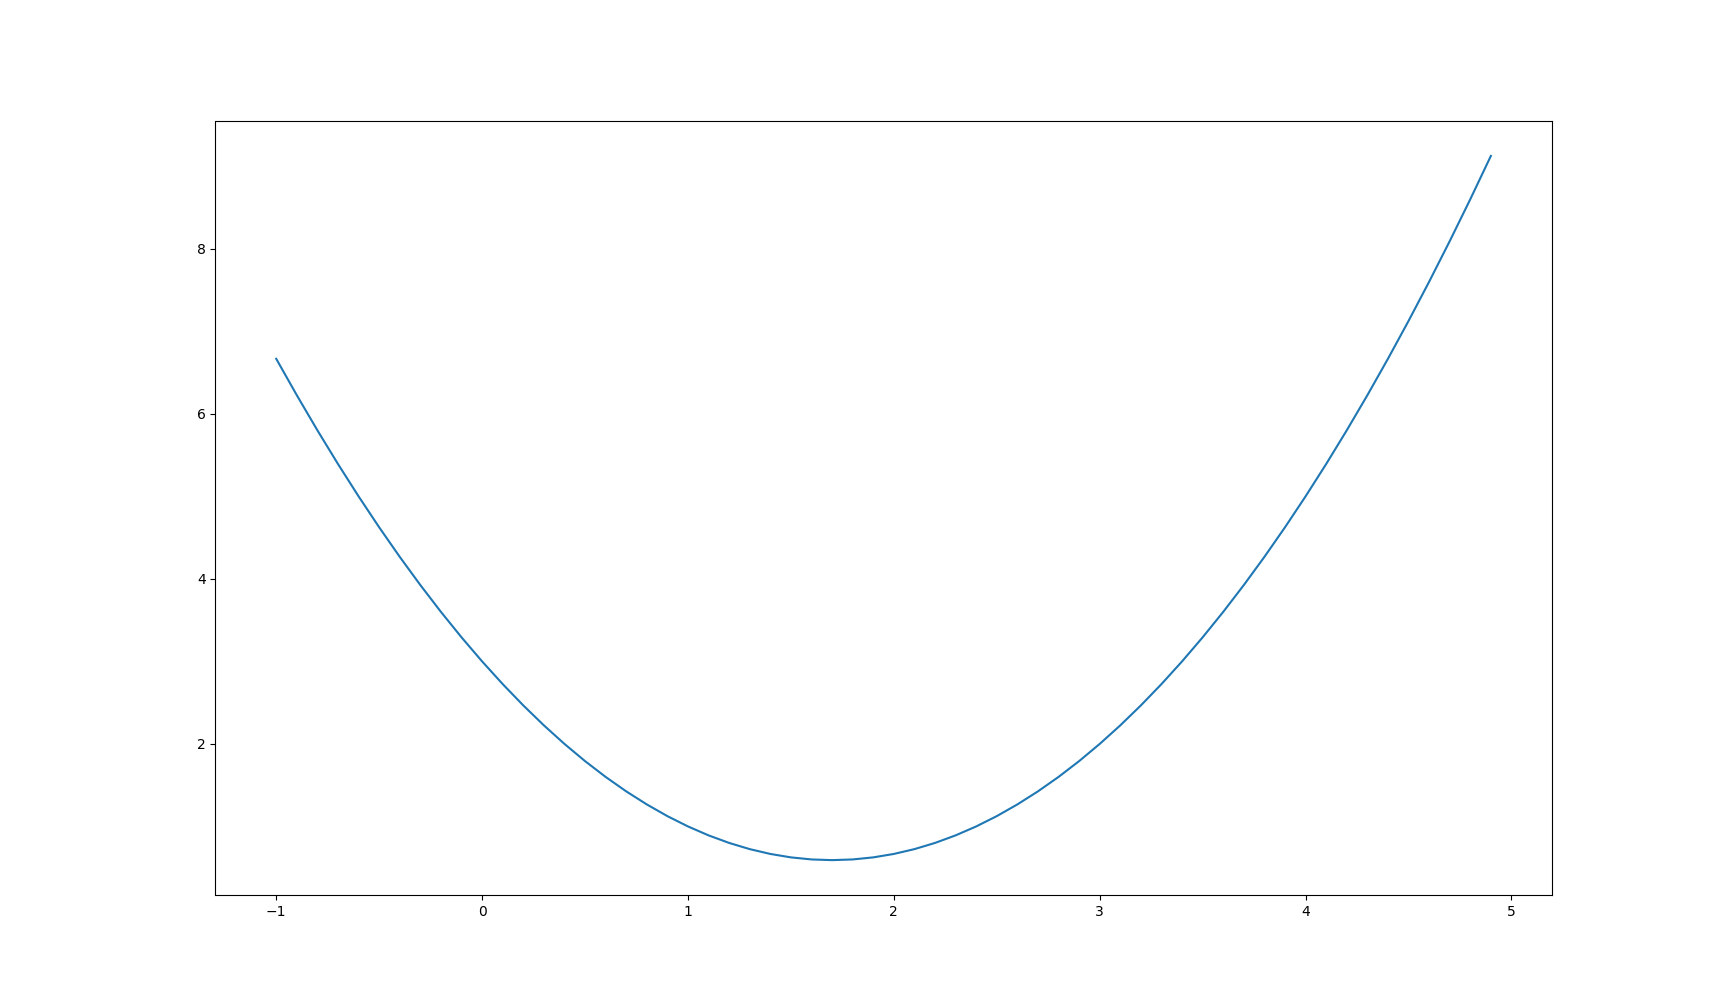
\includegraphics[keepaspectratio, scale=0.3]{lagrange1.png}
		\caption{ラグランジュ補間によって求めた関数の区間[-1,5]におけるグラフ}
	\end{figure}

	\subsection{課題2}
	$f(x)={(1+25{x^2}})^{-1}$を考える.区間$[-1,1]$において等間隔のデータを5点,11点,21点生成しそれぞれにラグランジュ補間を適用,そのグラフを示す.

	\begin{figure}[ht]
		\centering
		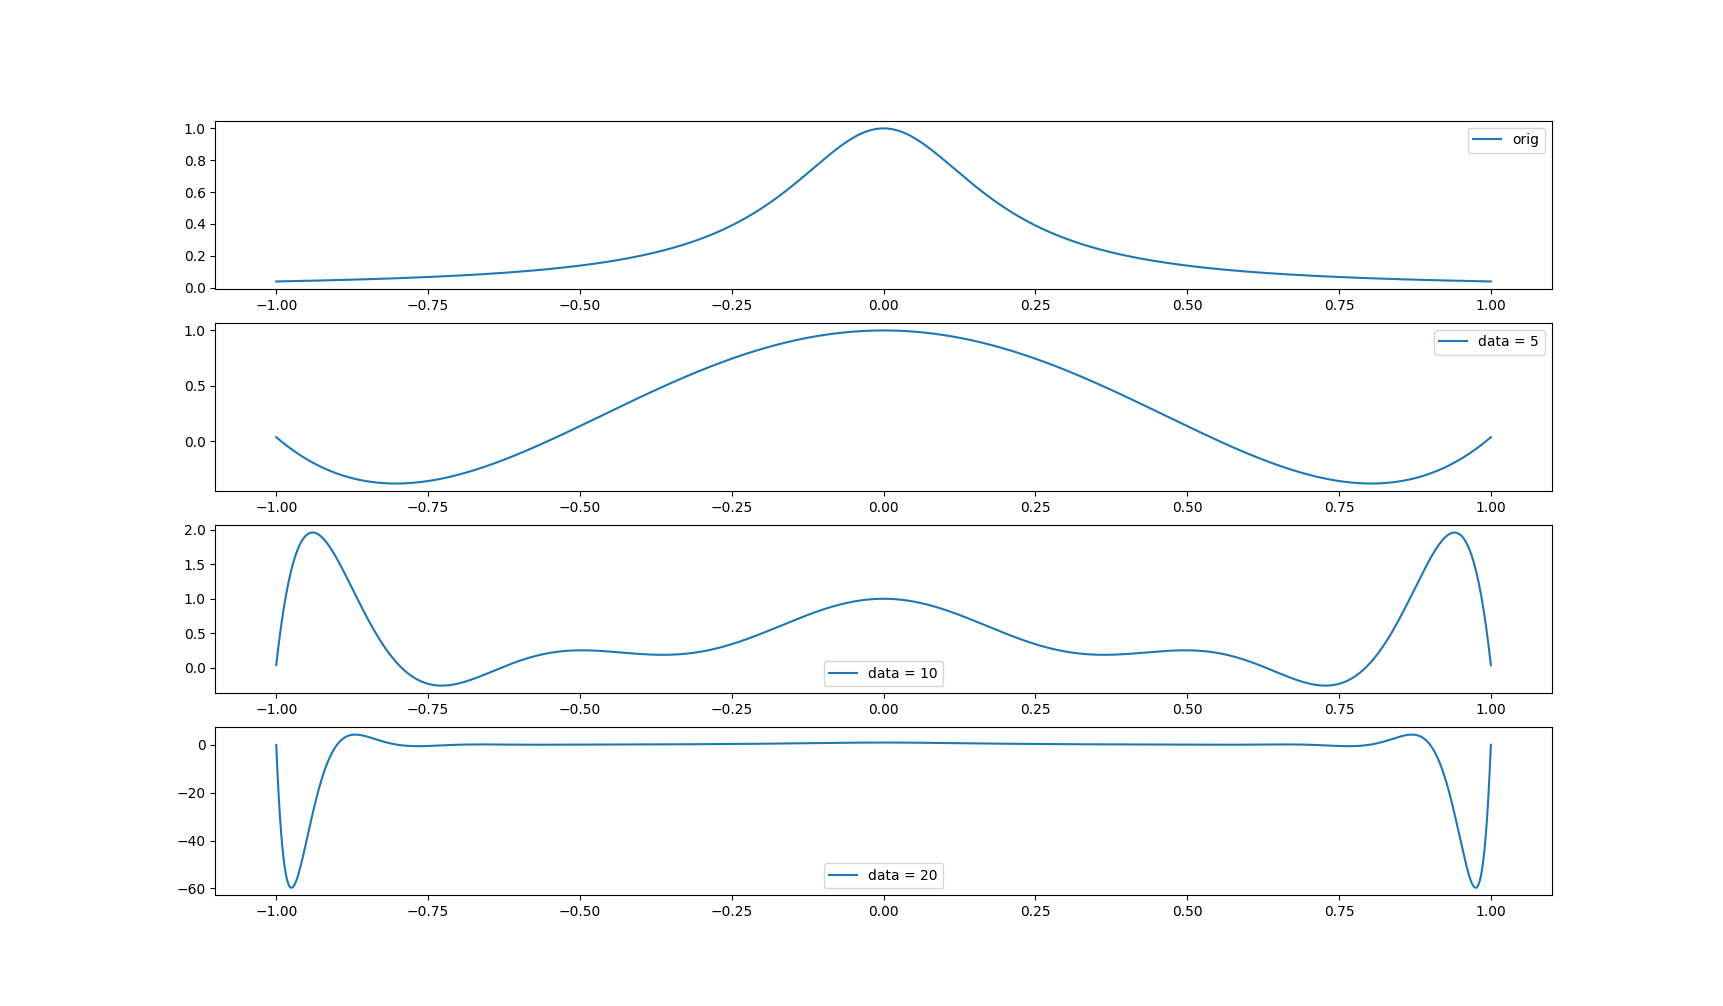
\includegraphics[keepaspectratio, scale=0.3]{lagrange2.png}
		\caption{上からデータ点が1000点,5点,11点,21点のときのグラフ}
	\end{figure}

	\section{付録}
	今回用いたソースコードを以下に示す.
	\subsection{課題1}
	\begin{lstlisting}
import numpy as np
import matplotlib.pyplot as plt

def lagrange(_x, _dataX, _dataY):
    l = 0
    L = 0
    for i in range(len(_dataX)):
        l = base(i, _x, _dataX) / base(i, _dataX[i], _dataX)
        L += _dataY[i] * l
    return L

def base(_i, _x, _dataX):
    l = 1
    for k in range(len(_dataX)):
        if _i != k:
            l *= _x - _dataX[k]
    return l

def main():
    dataX = np.array([1.0, 3.0, 4.0])
    dataY = np.array([1.0, 2.0, 5.0])

    x = np.arange(-1, 5, 0.1)
    y = lagrange(x, dataX, dataY)

    plt.plot(x, y)
    plt.show()

if __name__ == '__main__':
    main()
	\end{lstlisting}
	\subsection{課題2}
	\begin{lstlisting}
import numpy as np
import matplotlib.pyplot as plt

def func(_x):
    return 1 / (1 + 25 * (_x ** 2))

def lagrange(_x, _dataX, _dataY):
    l = 0
    L = 0
    for i in range(len(_dataX)):
        l = base(i, _x, _dataX) / base(i, _dataX[i], _dataX)
        L += _dataY[i] * l
    return L

def base(_i, _x, _dataX):
    l = 1
    for k in range(len(_dataX)):
        if _i != k:
            l *= _x - _dataX[k]
    return l

def main():
    xa = -1.0
    xb = 1.0

    step = (xb - xa) / 1000
    x = np.arange(xa, xb + step, step)
    y = func(x)

    step = (xb - xa) / 4
    dataX1 = np.arange(xa, xb + step, step)
    dataY1 = func(dataX1)
    L1 = lagrange(x, dataX1, dataY1)

    step = (xb - xa) / 10
    dataX2 = np.arange(xa, xb + step, step)
    dataY2 = func(dataX2)
    L2 = lagrange(x, dataX2, dataY2)
    
    step = (xb - xa) / 20
    dataX3 = np.arange(xa, xb + step, step)
    dataY3 = func(dataX3)
    L3 = lagrange(x, dataX3, dataY3)

    plt.subplot(411)
    plt.plot(x, y, label="orig")
    plt.legend()
    plt.subplot(412)
    plt.plot(x, L1, label='data = 5')
    plt.legend()
    plt.subplot(413)
    plt.plot(x, L2, label='data = 10')
    plt.legend()
    plt.subplot(414)
    plt.plot(x, L3, label='data = 20')
    plt.legend()
    plt.show()

if __name__ == '__main__':
    main()
	\end{lstlisting}
\end{document}
